%====================================================================
\frame{\frametitle{Self-exciting exponential Hawkes process} \label{back:Hawkes}

  $$
  \lambda(t)= \lambda_0 + a \underset{T_k < t}{\sum} e^{-b(t-T_k)}
  $$
  \paragraph{Self exciting:} 
  Each event increases the probability of observing another event
  
  \bigskip \bigskip \pause
  \begin{tabular}{cc}
    \hspace{-.04\textwidth}
    \begin{tabular}{p{.4\textwidth}}
%       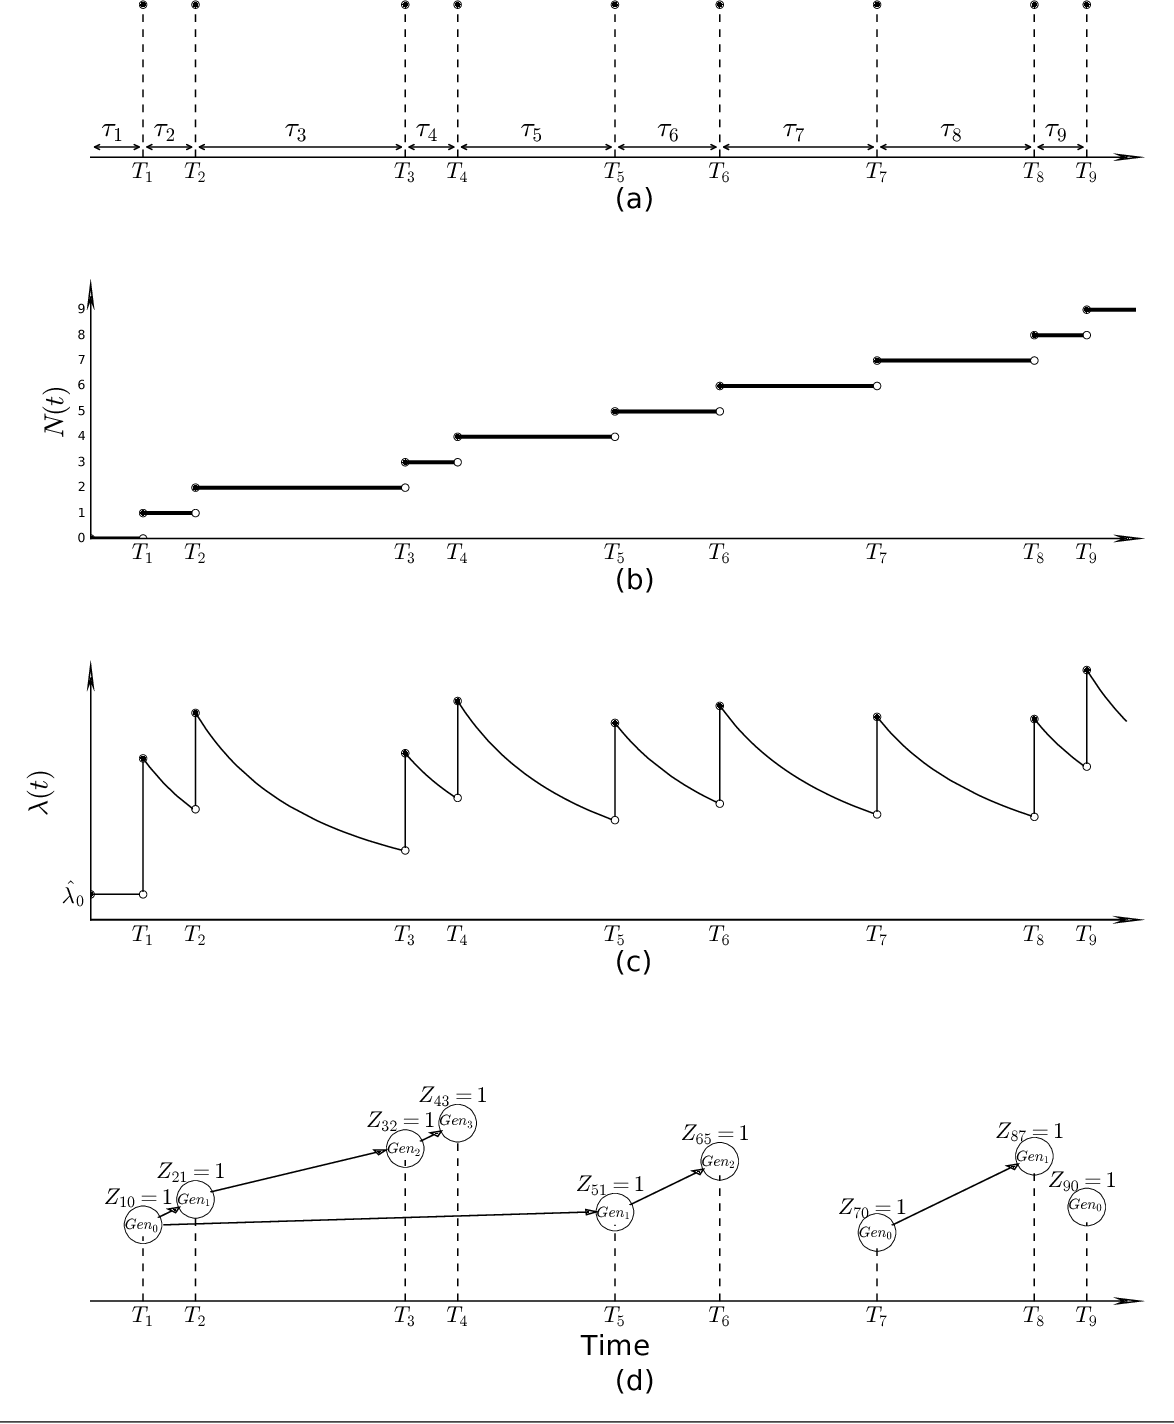
\includegraphics[width=.4\textwidth, trim=0 450 0 0, clip=]{\figcp/Bon24-Hawkes-Fig3}
      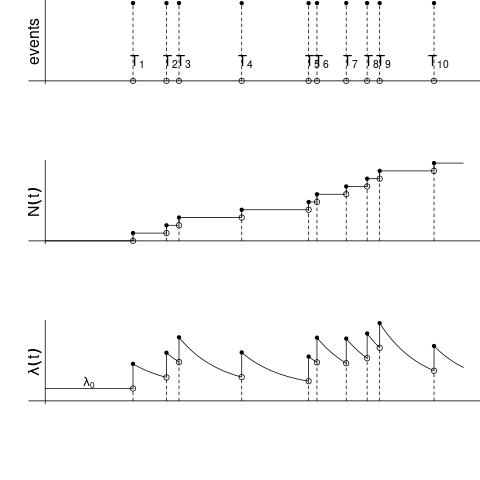
\includegraphics[width=.45\textwidth, trim=0 0 0 0, clip=]{\figcp/FigHawkes-intensity}
    \end{tabular}
    & 
%     \hspace{-.05\textwidth}
    \begin{tabular}{p{.55\textwidth}}
      \begin{itemize}
        \setlength{\itemsep}{.75\baselineskip}
        \item Exponential kernel function \emphase{$h(t)= a e^{-b t}$}
        \item \emphase{$a \geq 0$} to ensure that $\lambda$ is non negative 
        \item \emphase{$a/b <1$} to ensure stationarity
        \item Applications: sismology, epidemiology, vulcanology, neurosciences, ecology, ...
        \goto{sec:Hawkes}
      \end{itemize}
      ~ \\ ~ \\~ \\
    \end{tabular}
  \end{tabular}  

}

%====================================================================
\frame{\frametitle{Simulations: estimation} \label{back:HawkesFit}

  $$
  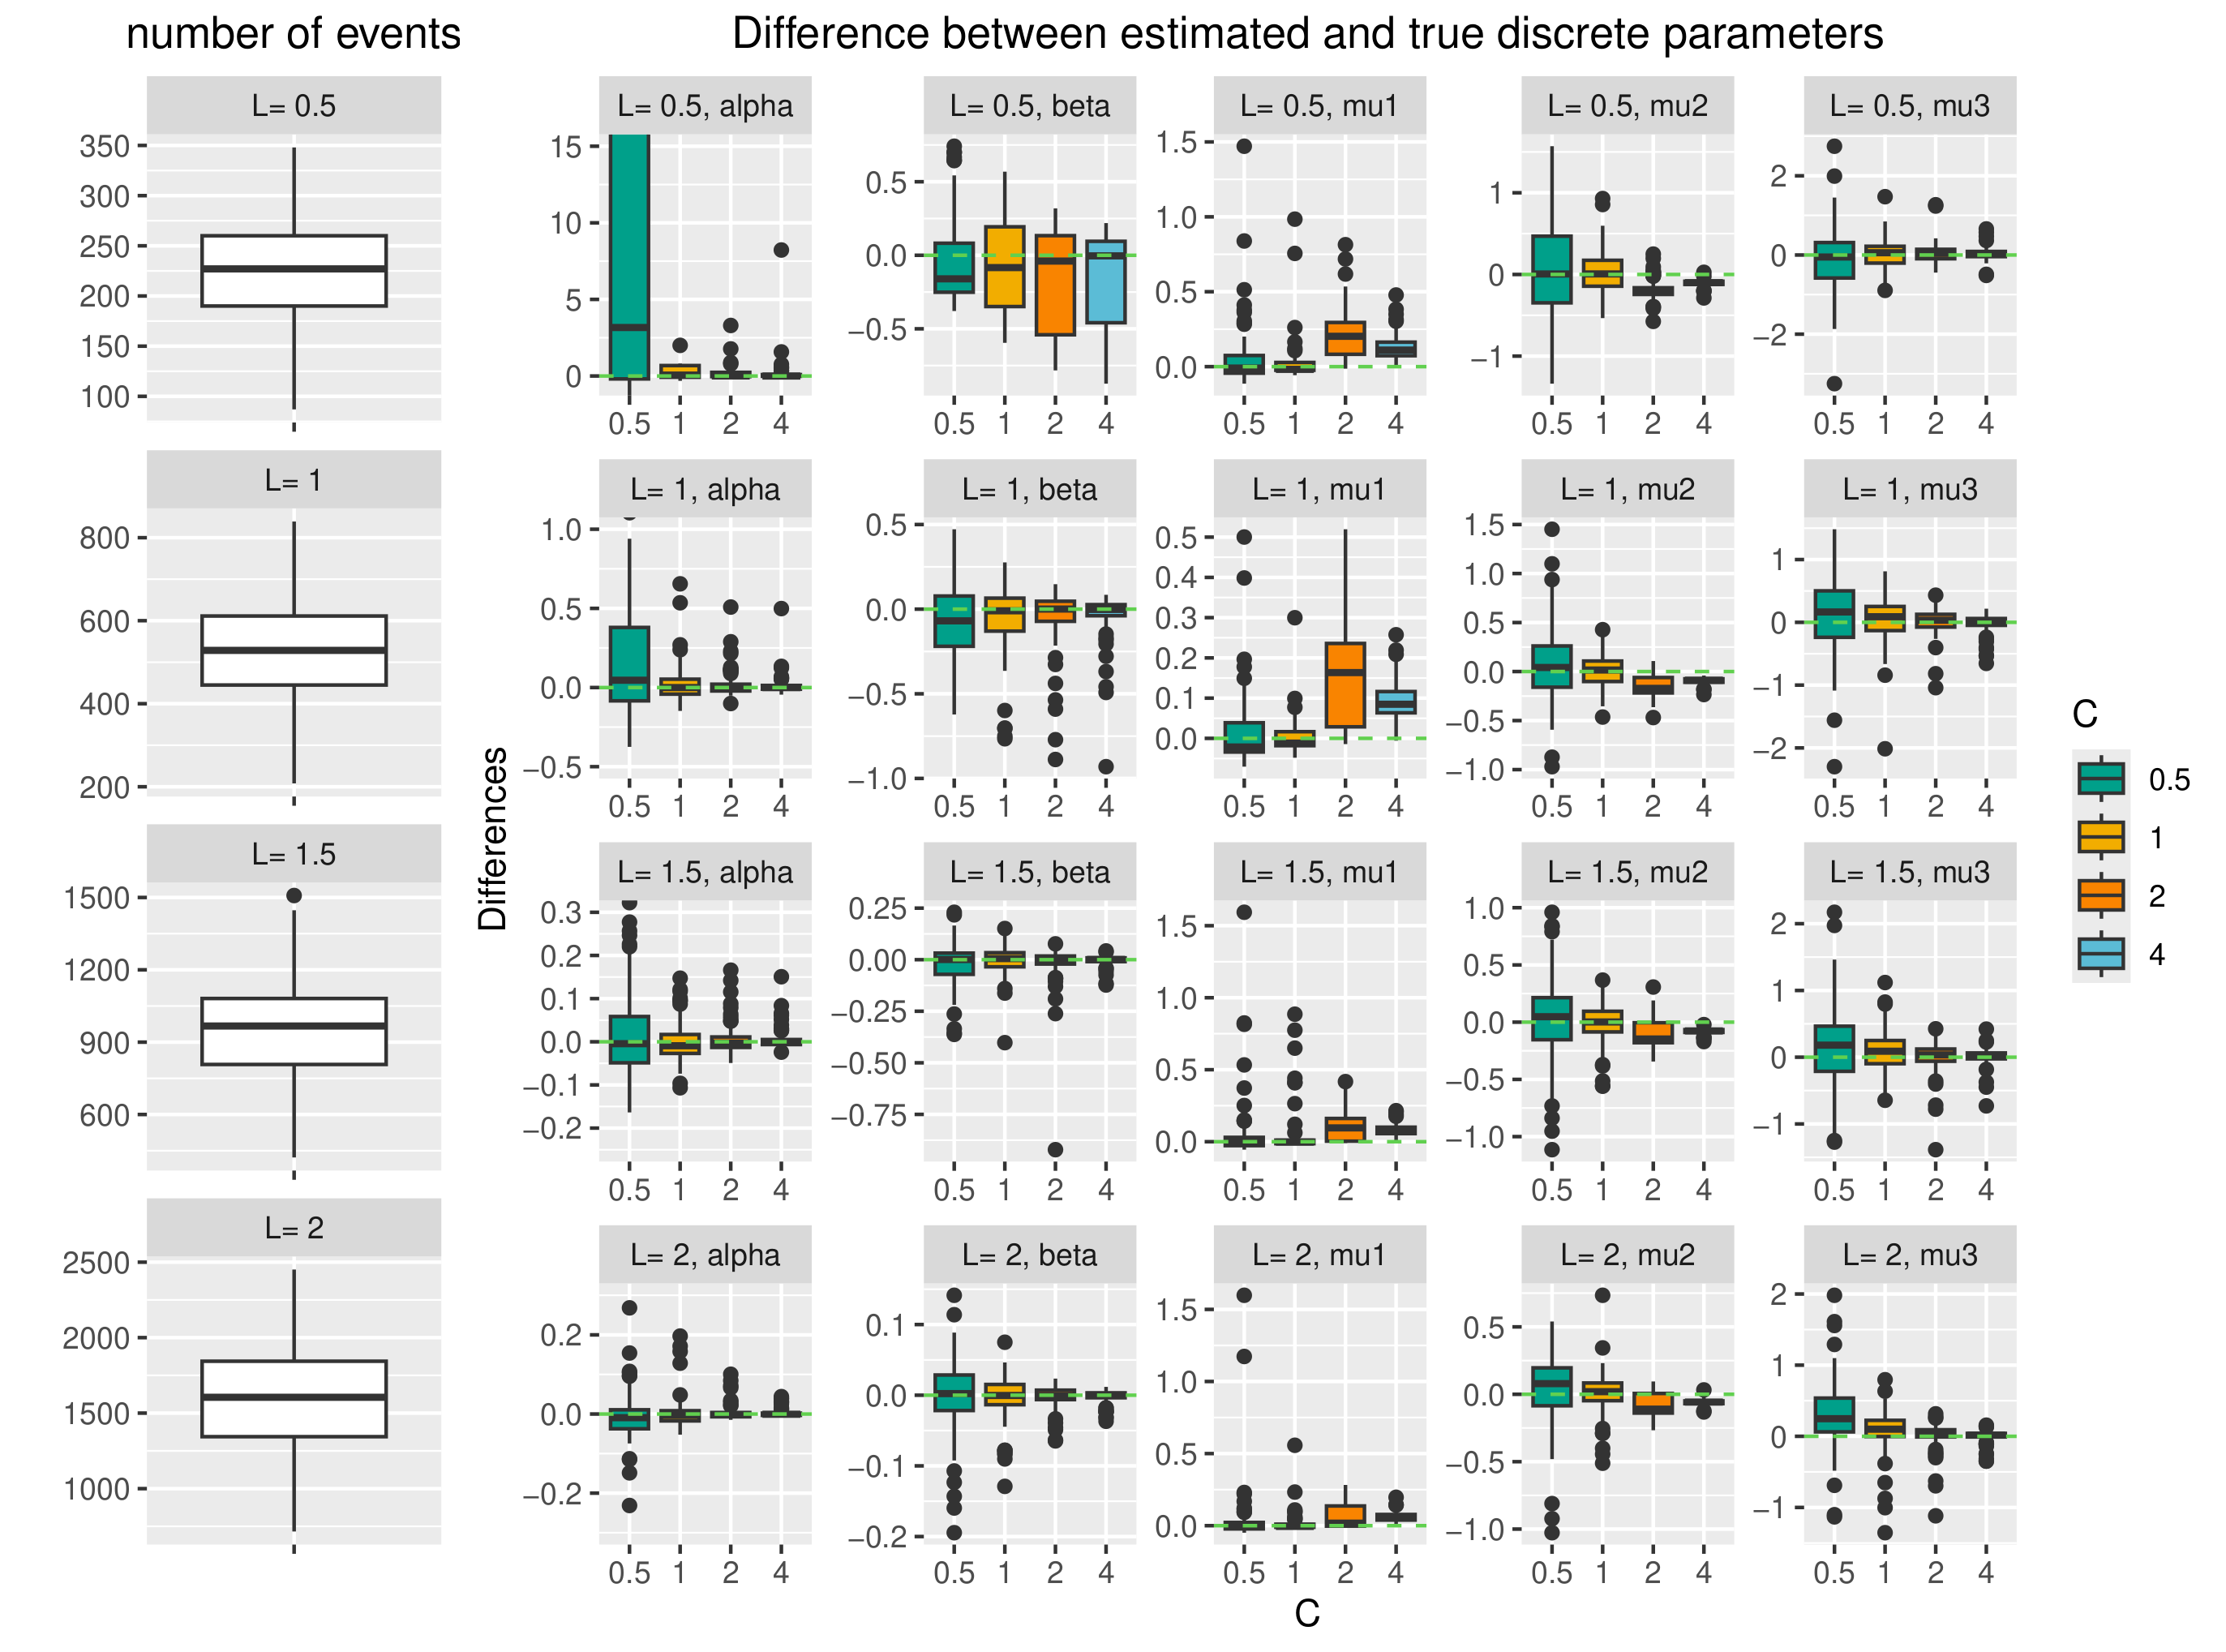
\includegraphics[width=0.75\textwidth]{\figcp/BoR25-ArXiv-disc_parm_scale_ggplot_V8_Q3}
  $$
  \goto{sec:HawkesSimuls}
}

%====================================================================
\frame{\frametitle{Simulations: model selection} \label{back:HawkesAIC}

  $$
  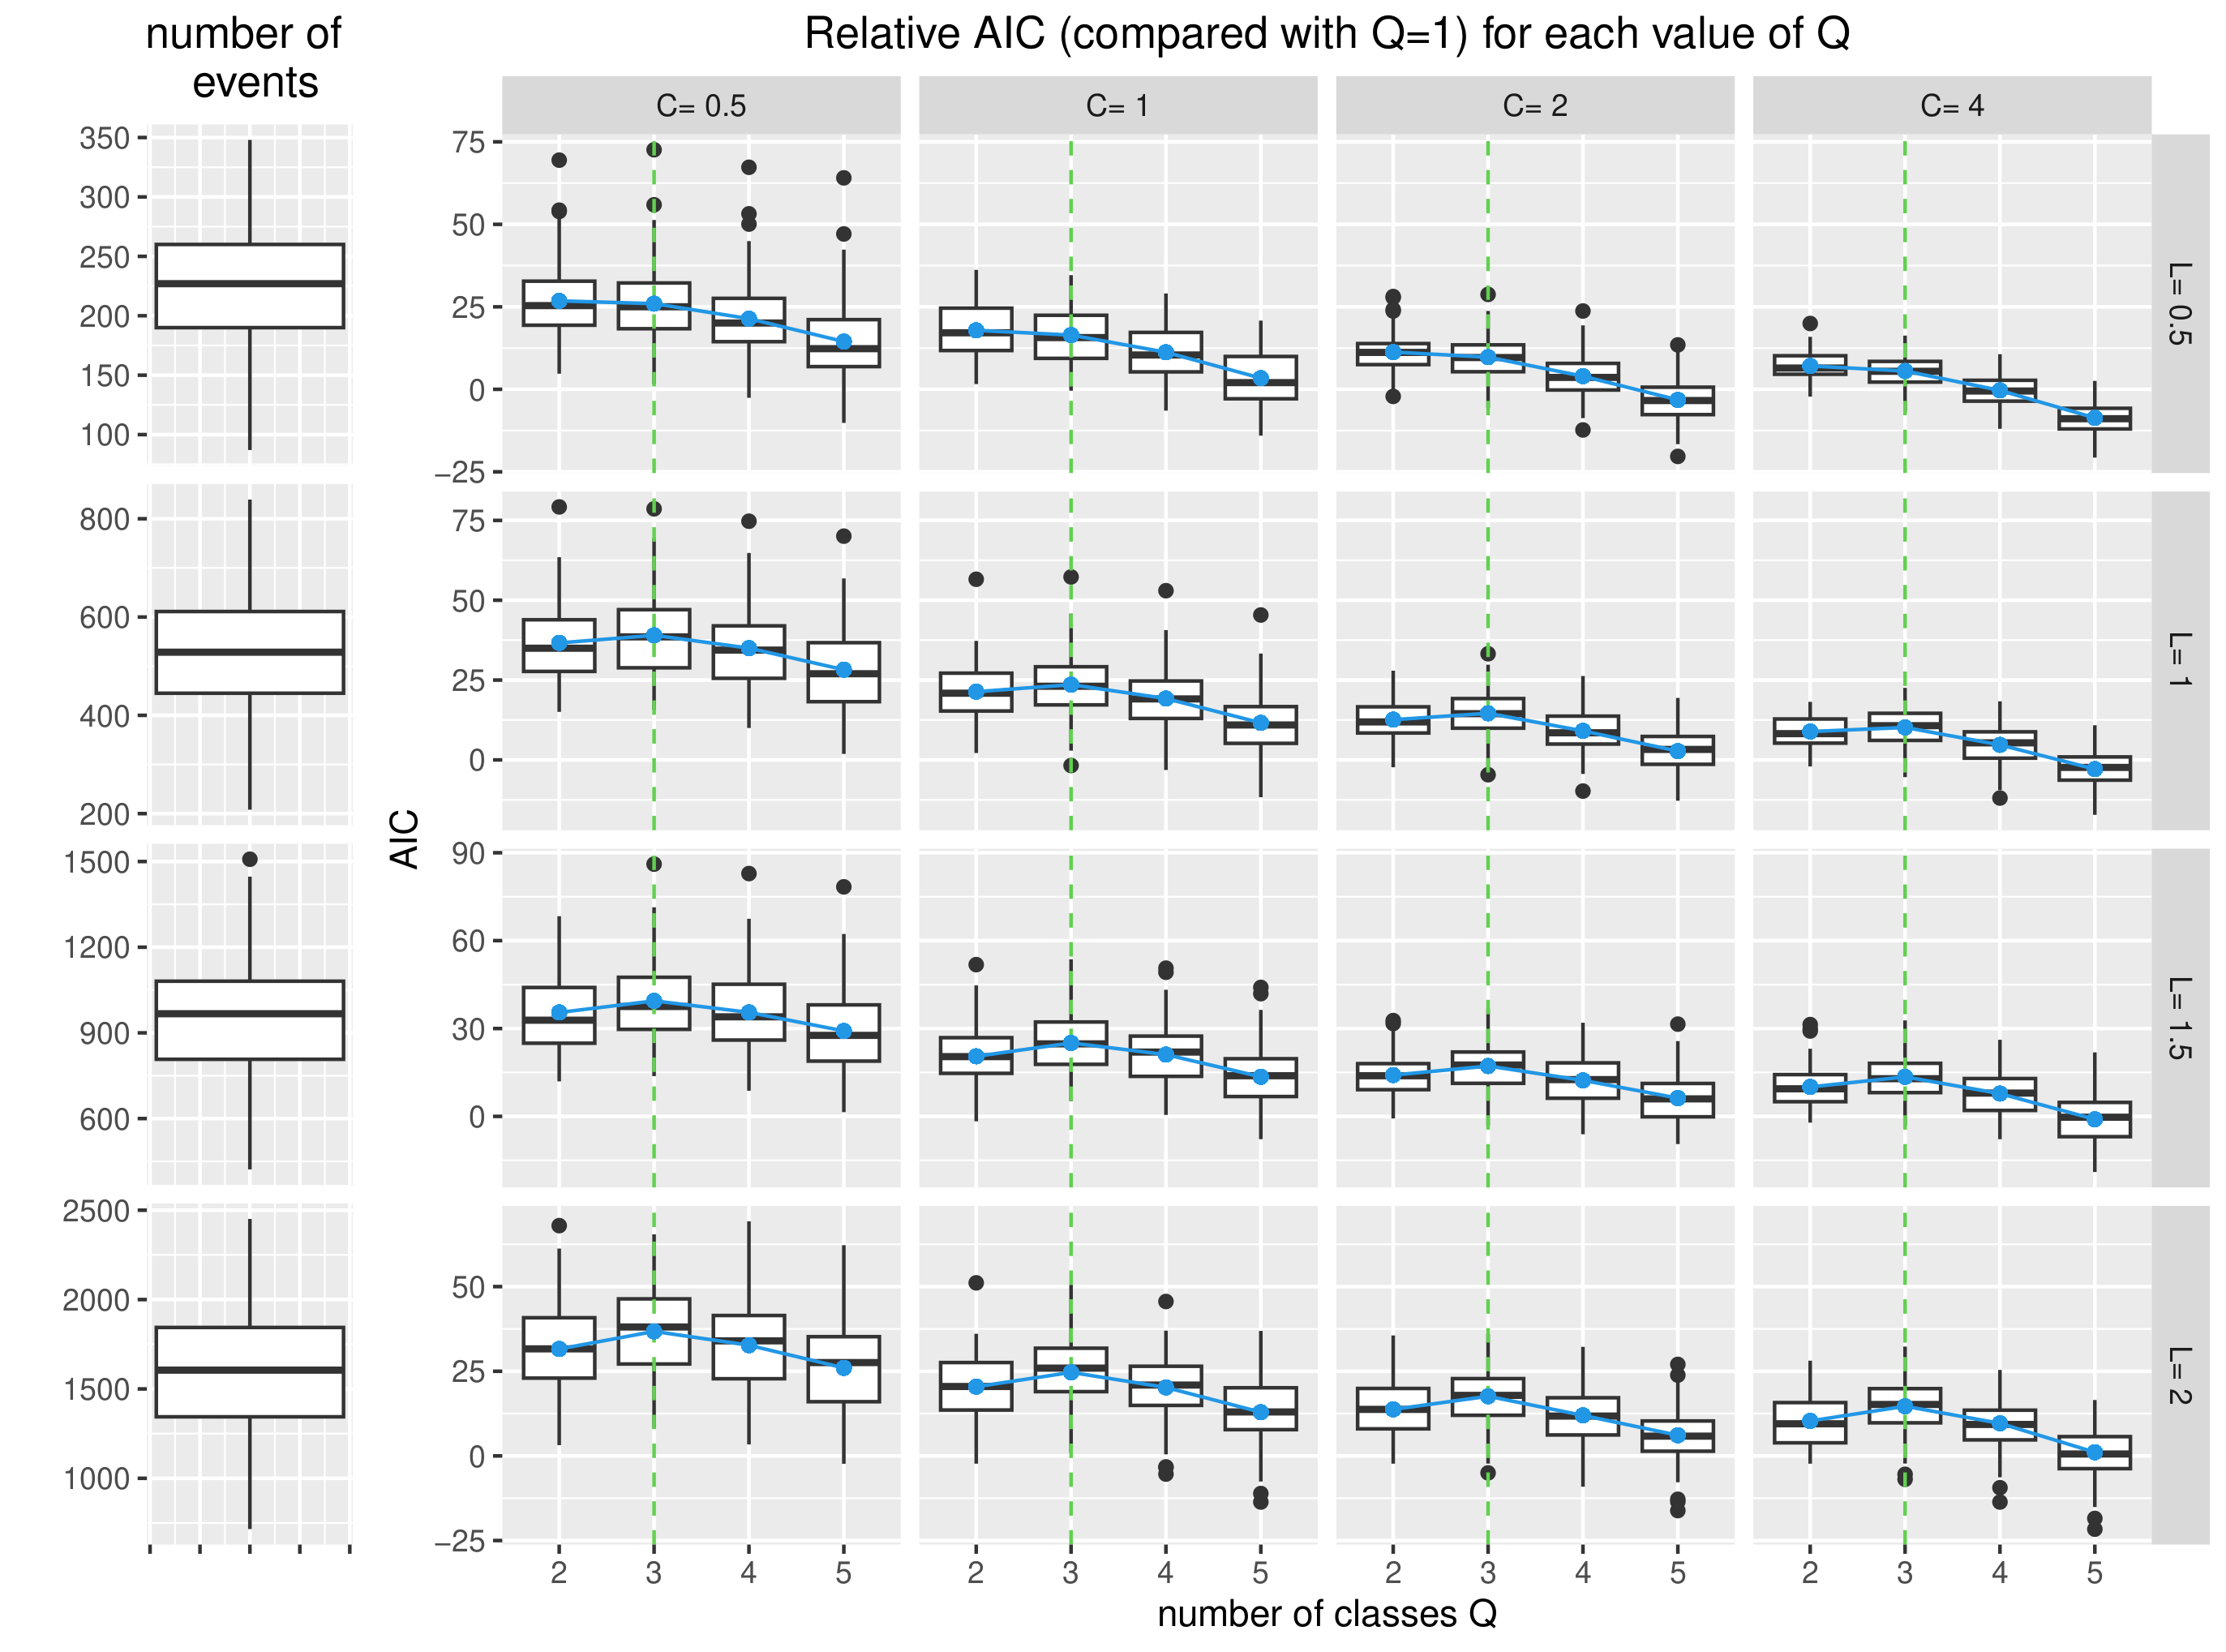
\includegraphics[width=0.75\textwidth]{\figcp/BoR25-ArXiv-aic_ggplot_V8_Q3}
  $$
  \goto{sec:HawkesSimuls}

}

%====================================================================
\frame{\frametitle{Simulations: classification and computational time} \label{back:HawkesClassif}

  $$
  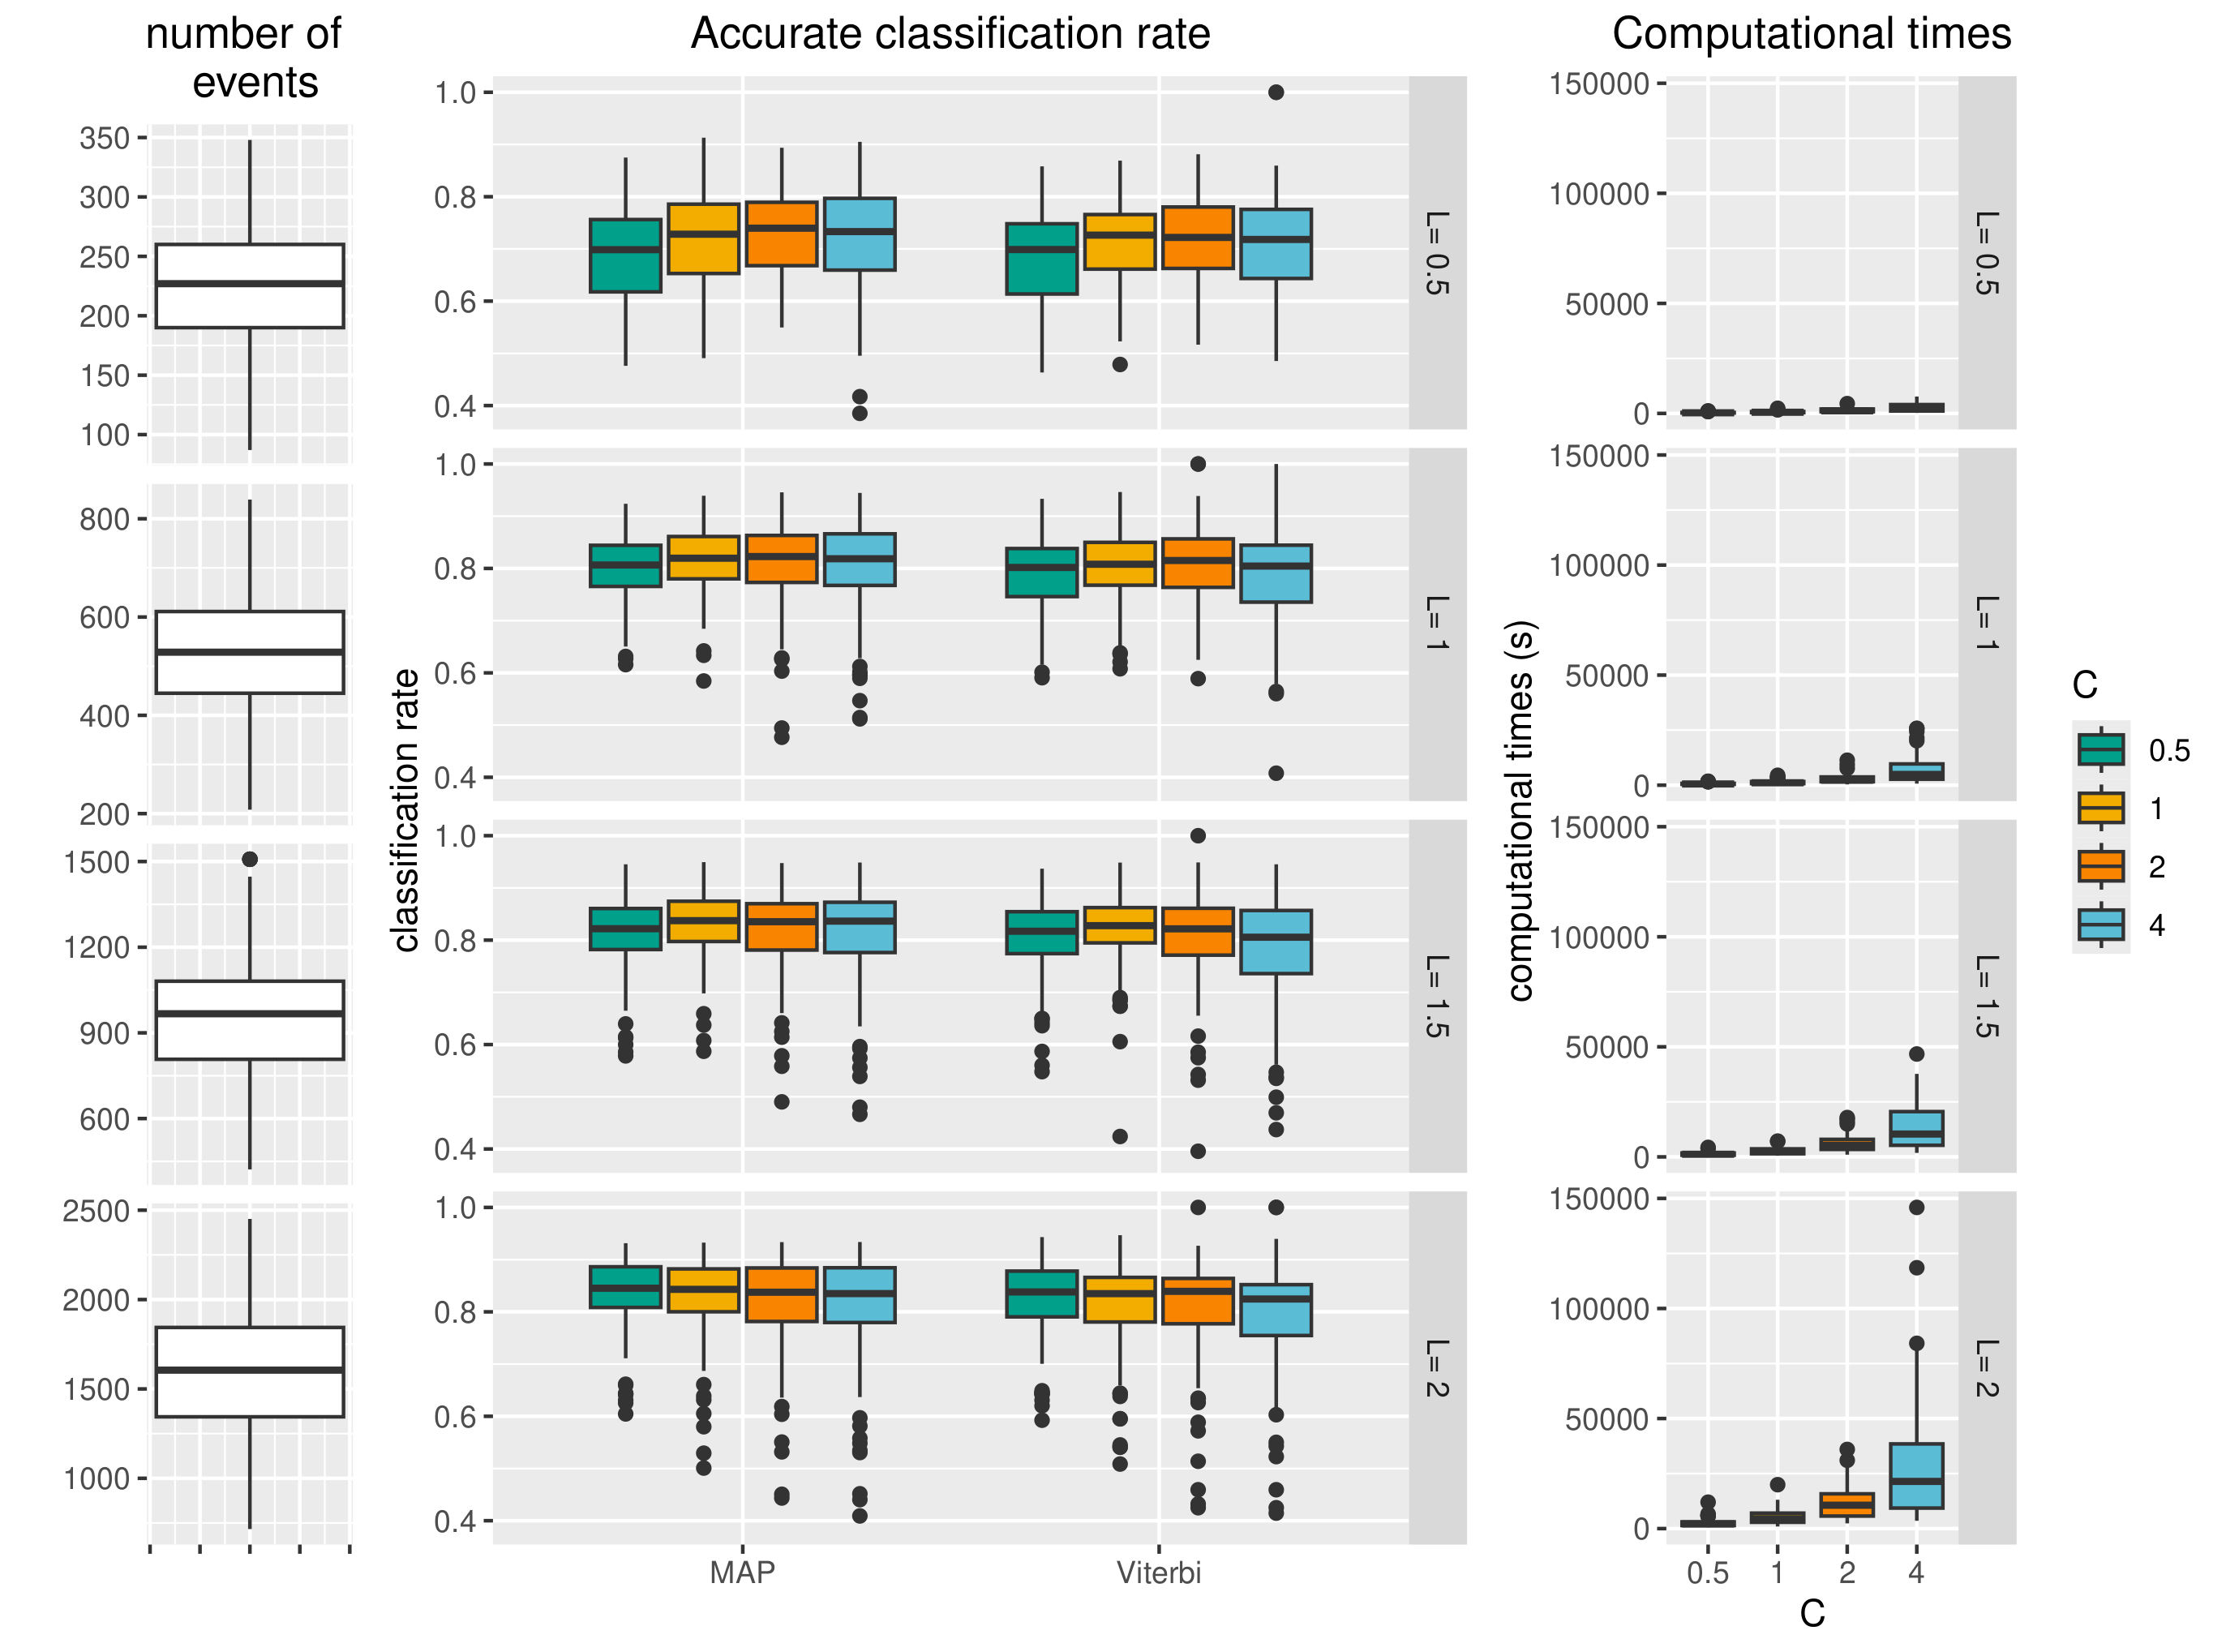
\includegraphics[width=0.75\textwidth]{\figcp/BoR25-ArXiv-classif_cpu_ggplot_V8_Q3}
  $$
  \goto{sec:HawkesSimuls}

}

%====================================================================
\frame{ \frametitle{Non exponential kernel function $h$} \label{back:HawkesKernel}

  \paragraph{Compact support.} 
  Suppose that $h$ has no exponential form, but 
  $$
  t > L \Delta
  \qquad \Rightarrow \qquad 
  h(t) = 0.
  $$

  \bigskip \bigskip 
  \paragraph{Homogeneous discrete Hawkes process.} 
  $$
  \left(Y_k \mid Y_{1:(k-1)}\right) \sim \Pcal\left(\mu + \sum_{\ell=1}^{k-1} \alpha_\ell Y_{k-\ell}\right) 
  \qquad \text{with} \quad
  \alpha_\ell = \int_{(\ell-1)\Delta}^{\ell\Delta} h(t) \d t.
  $$

  \bigskip \bigskip 
  \paragraph{Markovian representation.} 
  Define $U_k = \sum_{\ell \geq 1} \alpha_\ell Y_{k-\ell}$,
  then
  $$
  \left(Y_k \mid Y_{1:(k-1)}\right)
  = \left(Y_k \mid U_k\right) 
  \sim \Pcal\left(\mu + U_k\right)
  $$
  and $\left((Y_k, U_k)\right)_{k \geq 1}$ forms a Markov chain (of order $L$).
  
}
